\documentclass{beamer}
\usepackage[utf8]{inputenc}
\usepackage[T1]{fontenc}
\usepackage[french]{babel}
\usepackage{listings}
\usepackage{graphicx}
\usepackage{color}
\definecolor{vertc}{RGB}{235,241,221}
\lstset{language=Python,basicstyle=\ttfamily\footnotesize,%
        stringstyle=\ttfamily\color{brown},commentstyle=\color{blue},
        keywordstyle=\color{purple},
        backgroundcolor=\color{vertc}, frame=single, tabsize=2,
        breaklines=true, breakatwhitespace=false
}
\author{GConfs}
\title[Journée de découverte des métiers de l’ingénieur]{Atelier de découverte
de la programmation\\

\includegraphics[scale=0.2]{img/gconfs}
}
\usetheme{Hannover}
\begin{document}
\maketitle
\section{La programmation}
\begin{frame}{Exprimer vos désirs à la machine}
\emph{Computers are stupid. Learn to be stupid, and you’ll master them.}
\footnote{Dr. \textit{Cleymans S.}, 1991, \textit{Golden-eyed
scientists}, p.42}
\end{frame}
\begin{frame}{De l’humain à la machine : les deux mondes}
    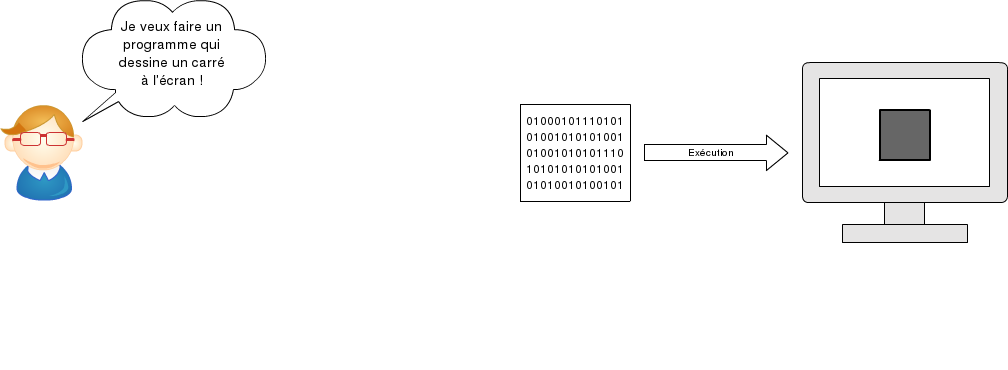
\includegraphics[scale=0.3]{img/cacoo0}
\end{frame}
\begin{frame}{De l’humain à la machine : un pas vers la machine}
    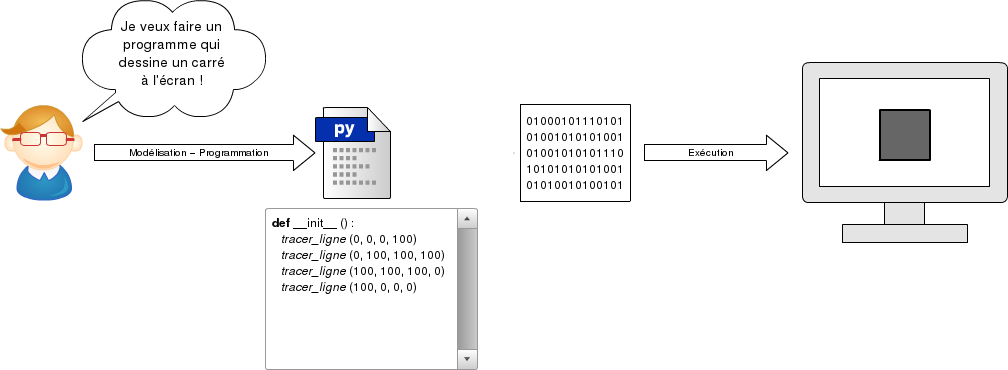
\includegraphics[scale=0.3]{img/cacoo1}
\end{frame}
\begin{frame}{De l’humain à la machine : le traducteur}
    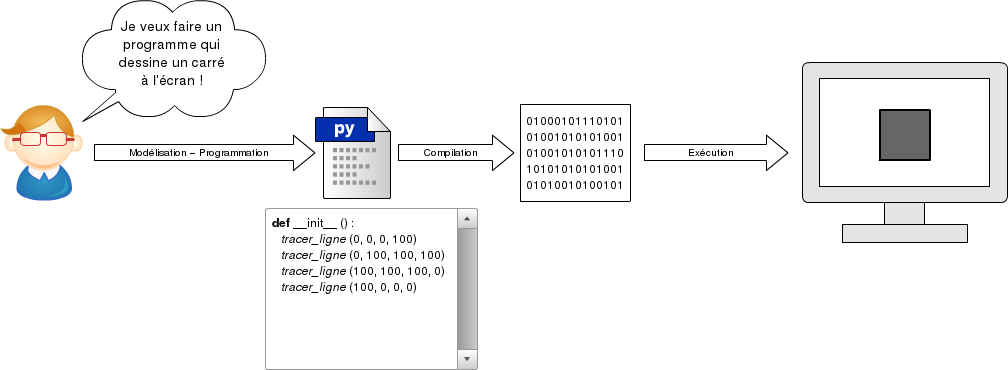
\includegraphics[scale=0.3]{img/cacoo}
\end{frame}
\section{Le python}
\subsection{Structures de base}
\subsubsection{Généralités}
\begin{frame}{Généralités}
\begin{block}{Langage simple}
    \begin{itemize}
        \item Interprété
        \item Syntaxe allégée
        \item Peu de contraintes de typage
        \item Code naturellement lisible
    \end{itemize}
\end{block}
\begin{block}{Langage omniprésent}
    \begin{itemize}
        \item Utilisable sur toutes les plateformes
        \item Utilisé dans l’industrie
    \end{itemize}
\end{block}
\end{frame}

\subsubsection{Les bases du langage}
\begin{frame}[fragile]{Les variables}
\begin{lstlisting}
    nom = "Login"
    prenom = "Xavier"
    pseudonyme = "login_x"
    age = 20
    poids = 63.30
\end{lstlisting}
\end{frame}

\begin{frame}[fragile]{Les procédures}
\begin{itemize}
\item Appel de procédure :\\
\begin{lstlisting}
tourner_droite (100)
\end{lstlisting}
\item Déclaration de procédure :\\
\begin{lstlisting}
 def tourner_droite (angle) :
     mon_orientation = orient_courante + angle
\end{lstlisting}
\end{itemize}
\end{frame}

\begin{frame}[fragile]{Les boucles}
\begin{itemize}
\item Boucle avec variable :
    \begin{lstlisting}
    for i in range (4) :
       print (42)
    \end{lstlisting}
    Sortie : \verb+42 42 42 42+
\item Boucle avec intervalle et incrément :
    \begin{lstlisting}
    for i in range (4, 6, 1) :
       print (i)
    \end{lstlisting}
    Sortie : \verb+4 5+
\end{itemize}
\end{frame}

\subsection{Pratiquer pour régner}
    \begin{frame}{Dessiner avec une tortue}
    \begin{itemize}
    \item État initial\\
    
\includegraphics[width=40px,height=20px]{img/square_0}

    \item avancer (200)\\
    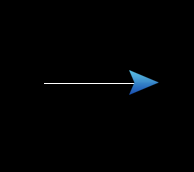
\includegraphics[width=40px,height=20px]{img/square_1}

    \item tourner\_gauche (90)\\
    
\includegraphics[width=40px,height=20px]{img/square_2}

    \item avancer (100)\\
    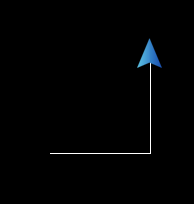
\includegraphics[width=40px,height=20px]{img/square_3}

    \item Et ainsi de suite\\
    
\includegraphics[width=40px,height=20px]{img/square_final}
    \end{itemize}
    \end{frame}
    \begin{frame}
    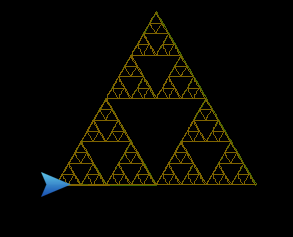
\includegraphics{img/sierpinski}
    \end{frame}
\end{document}
